% !TEX root = ../main.tex
\subsubsection{Central Detector} \label{sssec::centraldetector}
    Particles scattered from the target at polar angles in the range from $35\degree$ to $125\degree$ are detected in the CD with its own particle identification and tracking detectors.
    Charged particles are tracked in the Central Vertex Tracker (CVT) and detected in the Central Time-of-Flight (CTOF) detector with full coverage in azimuthal angle.
    Neutron detection is provided by the Central Neutron Detector (CND) located radially outside of the CVT and the CTOF.

% --+ CVT +---------------------------------------------------------------------
\paragraph{Central Vertex Tracker (CVT)}
    The CVT system is a part of the CD and is used to measure the momentum and to determine the vertex of charged particles scattered from the target.
    The tracker lies inside the solenoid magnet, as can be seen in Figure \ref{fig::cvt}.
    CVT consists of two separate detectors, a Silicon Vertex Tracker (SVT) and a
    Barrel MicroMegas Tracker (BMT).

    The SVT system includes three regions with 10, 14, and 18 double-sided modules of silicon sensors instrumented with a digital ASIC readout.
    The readout pitch is \SI{156}{\micro\metre}, and the total number of channels is 21,504 \cite{antonioli2020}.

    The BMT contains three layers of strips along the beamline and three layers of circular readout strips around the beamline, with a total number of 15,000 readout elements.
    The BMT provides important improvements in momentum resolution and in tracking efficiency.
    Each layer is arranged azimuthally in three segments of $120\degree$ azimuthal coverage each.
    The system operates at the full design luminosity of $10^{35} \text{cm}^{-2}\text{s}^{-1}$ \cite{acker2020mvt}.

    Another component of the CVT is the Forward MicroMegas Tracker (FMT), which consists of six layers with 6144 readout elements.
    It is integrated mechanically with the CVT to provide a compact tracking system, but covers the polar angle range from $5\degree$ to $35\degree$ and provides improved vertex reconstruction for forward-scattered charged particles \cite{acker2020mvt}.
    The FMT working principle and geometry are discussed in detail in Section \ref{sec::fmtalignmentandreconstruction}.

% --+ CTOF +--------------------------------------------------------------------
\paragraph{Central Time-of-Flight}
    \begin{wrapfigure}{r}{0.49\textwidth}
        \centering\frame{
        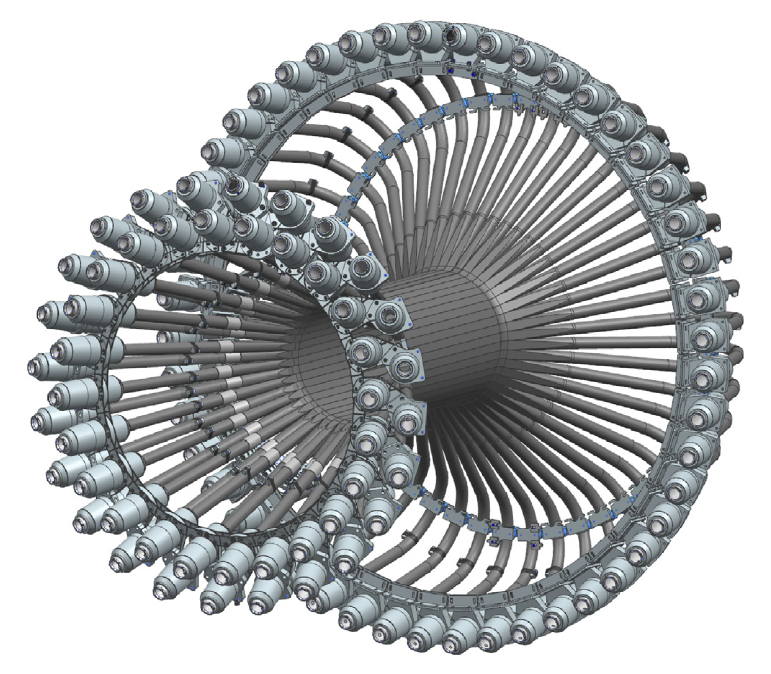
\includegraphics[width=\linewidth]{11experiment/img/22ctof.png}}
        \caption[Central Time-of-Flight]{Render of the Central Time-of-Flight.
        The render shows CTOF's 48 scintillator bars outfitted with light guides, PMTs, and magnetic shields at both ends of each counter.}
        \label{fig::ctof}
    \end{wrapfigure}

    The CTOF system is used for the identification of charged particles emerging from the target via TOF measurements in the momentum range from $0.3$ to about $1.25 ~\text{GeV}$.
    The CTOF includes 48 plastic scintillators with double-sided PMT readout via, respectively, 1.0-m-long upstream and 1.6-m-long downstream focusing light guides.
    The array of counters forms a hermetic barrel around the target and the CVT.
    The barrel is aligned with the beam axis inside the 5 T solenoid magnet.
    The PMTs are placed in a region of 0.1 T fringe field of the solenoid and enclosed within a triple layer dynamical magnetic shield that provides less than 0.2 G internal field near the PMT photocathode.
    The CTOF system is designed to provide time resolution of 80 ps for charged particle identification in the CLAS12 CD \cite{carman2020ctof}.
    A render of CTOF can be seen in figure \ref{fig::ctof}.

% --+ CND +---------------------------------------------------------------------
\paragraph{Central Neutron Detector (CND)}
    The CLAS12 CD is also equipped with the CND positioned radially outward of the CTOF.
    It allows the detection of neutrons in the momentum range from $0.2$ to $1.0 \text{GeV}$ by measurement of their TOF from the target and the energy deposition in the scintillator layers.
    The detector is made of three layers of scintillator paddles (48 paddles per layer), coupled two-by-two at the downstream end with semi-circular light guides.
    The signal is read out at the upstream end by PMTs placed outside of the high magnetic field region of the solenoid.
    The scintillators are connected to 1-m-long bent light guides \cite{chatagnon2020}.

% --+ BAND +--------------------------------------------------------------------
\paragraph{Back Angle Neutron Detector (BAND)}
    Neutron detection at back angles is accomplished with the BAND, which is positioned 3 metres upstream of the target.
    It detects backward neutrons with momenta between $0.25$ and $0.7$ GeV.
    The detector consists of 18 horizontal rows and five layers of scintillator bars with PMT readout on each end to measure TOF from the target.
    There is an additional $1 \text{cm}$ scintillation layer for vetoing charged particles.
    BAND covers a polar angle range from $155\degree$ to $175\degree$ with a design neutron detection efficiency of $35\%$ and a momentum resolution of about $1.5\%$ \cite{segarra2020}.
